% Desenho do sistema
\chapter{Desenho do sistema}
\label{cap3}

Os modelos propostos de interfaces com o utilizador, base de dados, classes e diagramas foram desenvolvidos no âmbito das disciplinas leccionadas até a data deste trabalho, reunindo assim neste trabalho todo um conjunto de aptidões e capacidades fundamentais para o desenvolvimento do sistema apresentado. Os pontos seguintes representam o trabalho desenvolvido e os métodos utilizados para o desenho do sistema.

\section{Modelação de interfaces}

Para o desenvolvimento das interfaces foram utilizados vários modelos, permitindo assim perceber de forma genérica as sequências de acções de navegação do utilizador. A figura \ref{fig:diagrama_arvore} representa uma árvore na qual podemos observar as páginas do portal e entender qual a ligação entre as diversas páginas utilizadas no portal.
É nossa intenção manter a simplicidade na estrutura do portal, optando por criar páginas simples que efectuem apenas uma função e não possuir "profundidade" de navegação.

\begin{figure}[!h]
	\centering
	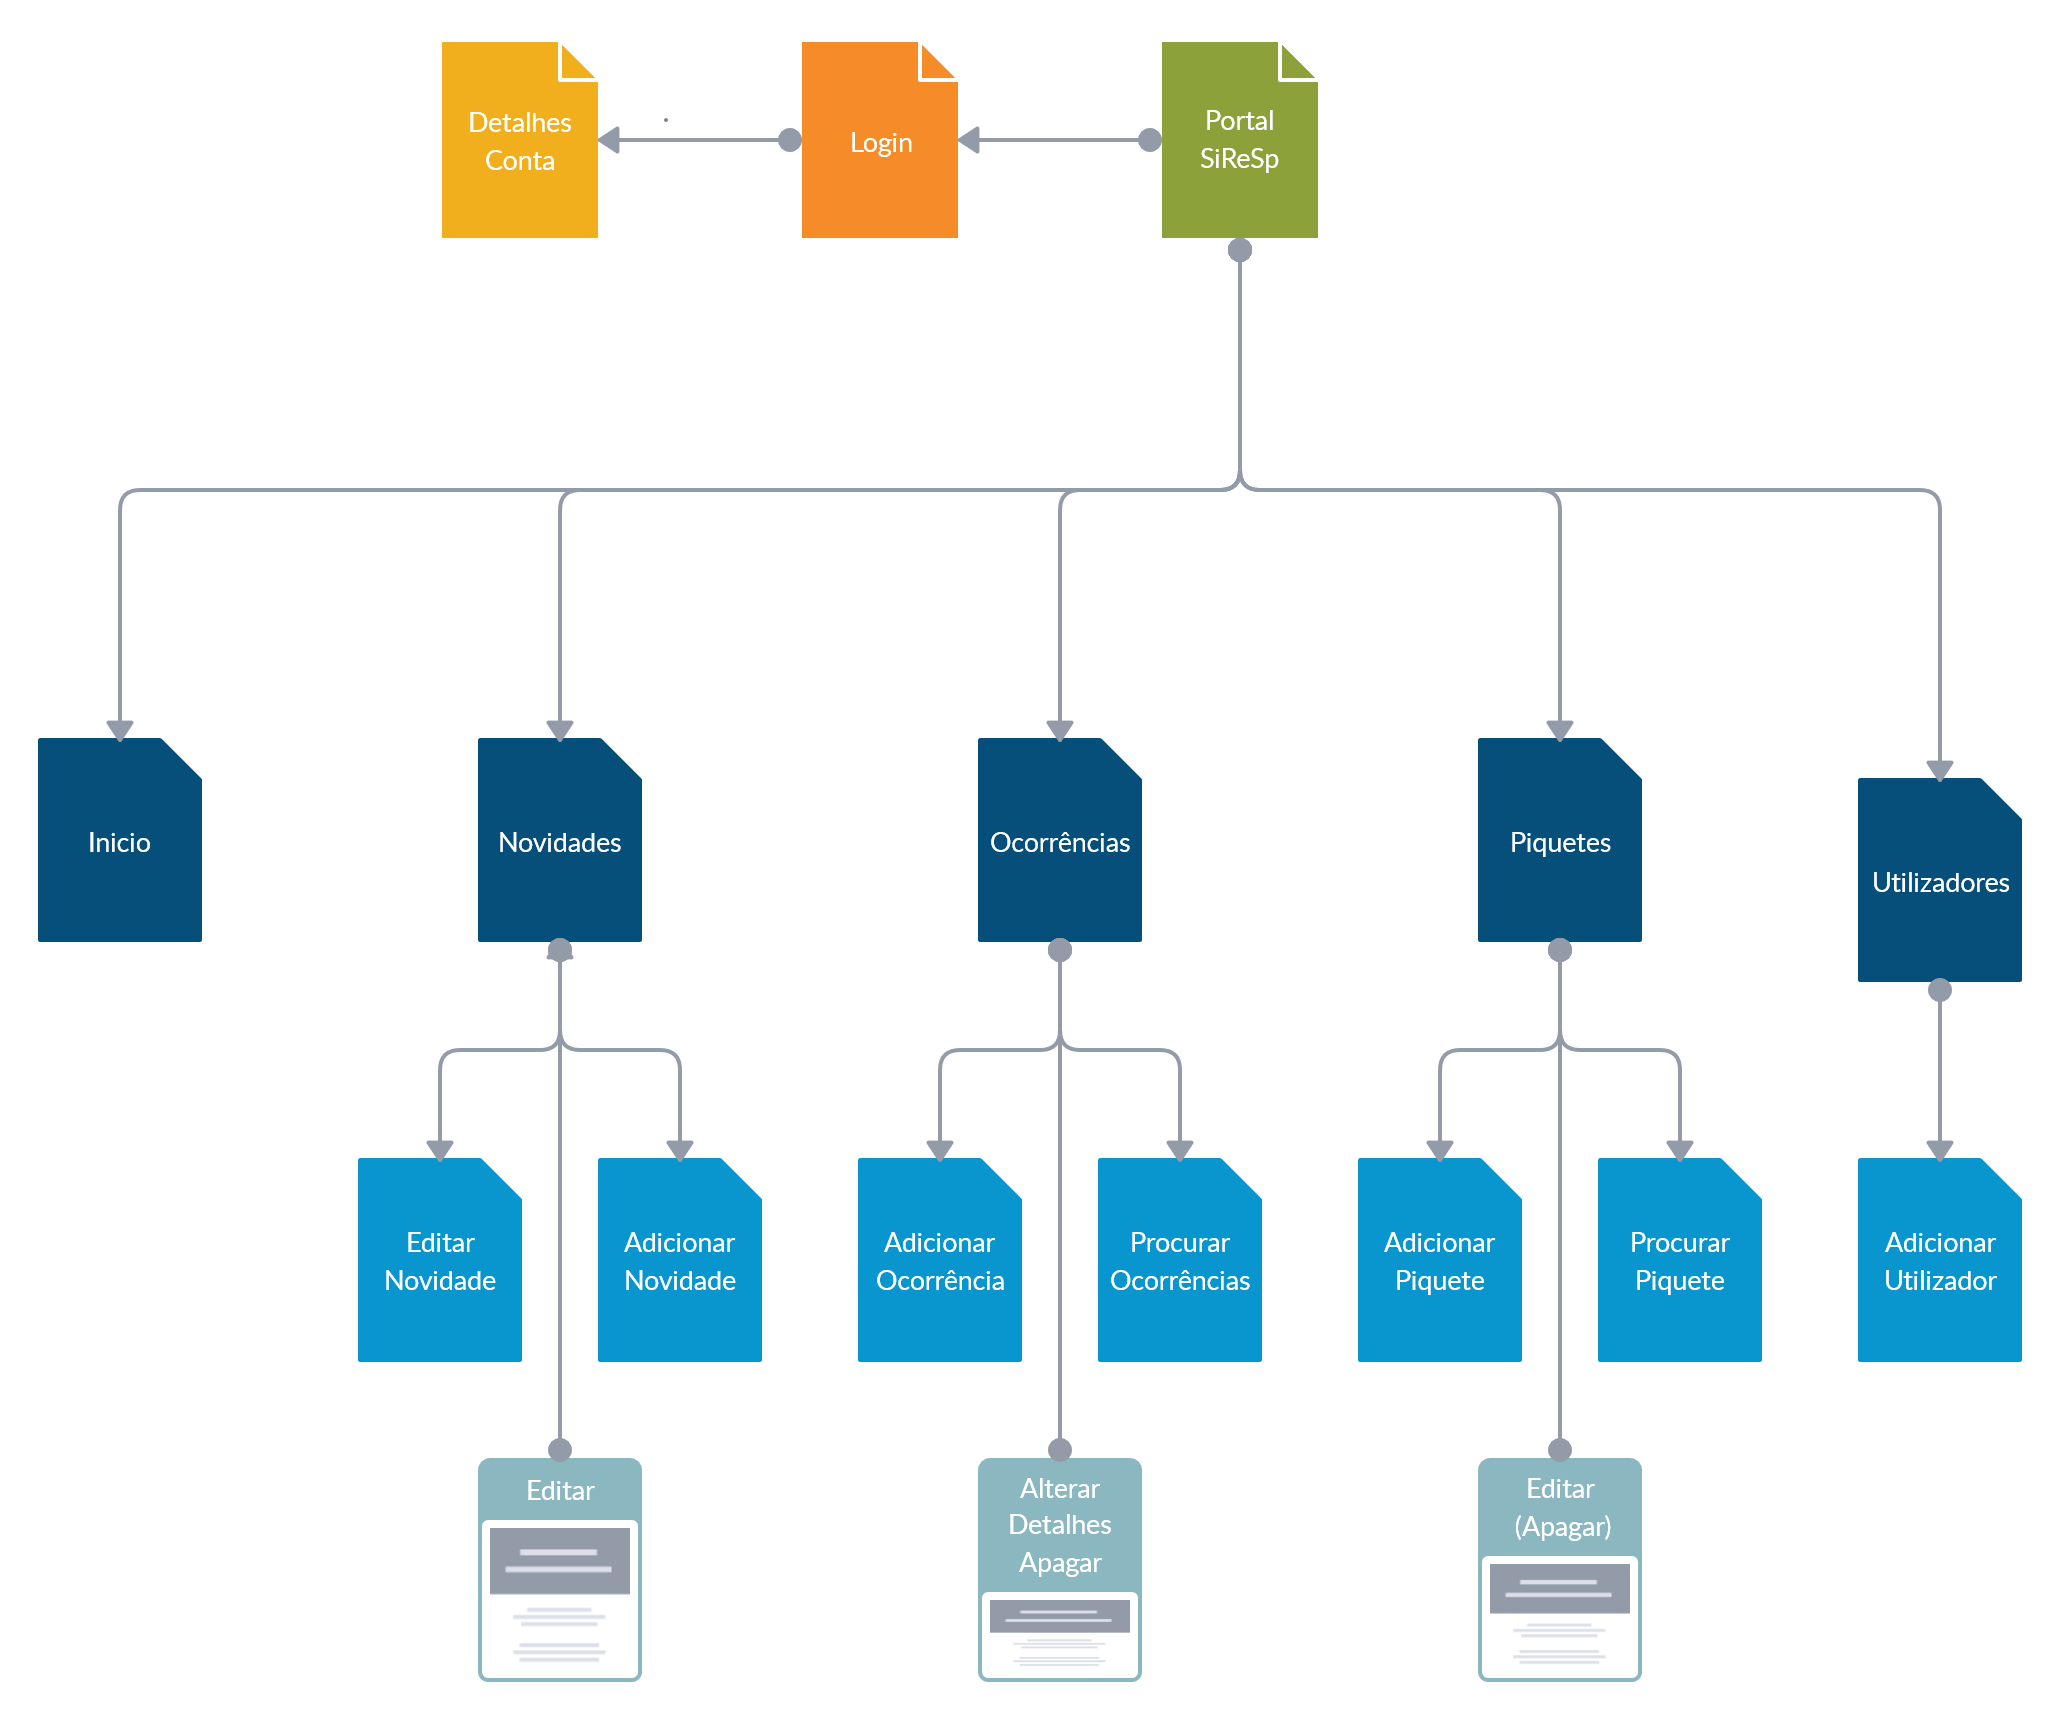
\includegraphics[width=\textwidth]{figuras/diagrama_arvore.png}
	\caption{Árvore de navegação no portal}
	\label{fig:diagrama_arvore}
\end{figure}

\FloatBarrier\subsection{Storyboard de navegação}

Apresentamos de seguida uma série de desenhos de baixa fidelidade, em papel, que tentam mostrar as informações e estrutura do portal.

\FloatBarrier
A figura \ref{fig:inicio} representa a página inicial do portal, onde é possível aceder Às opções login e visualizar a página de novidades. A navegação será sempre realizada por um menu horizontal com hiperligações no topo da página. A localização será sempre dada pelo título da página aberta no explorador.
\begin{figure}[!htb]
	\centering
	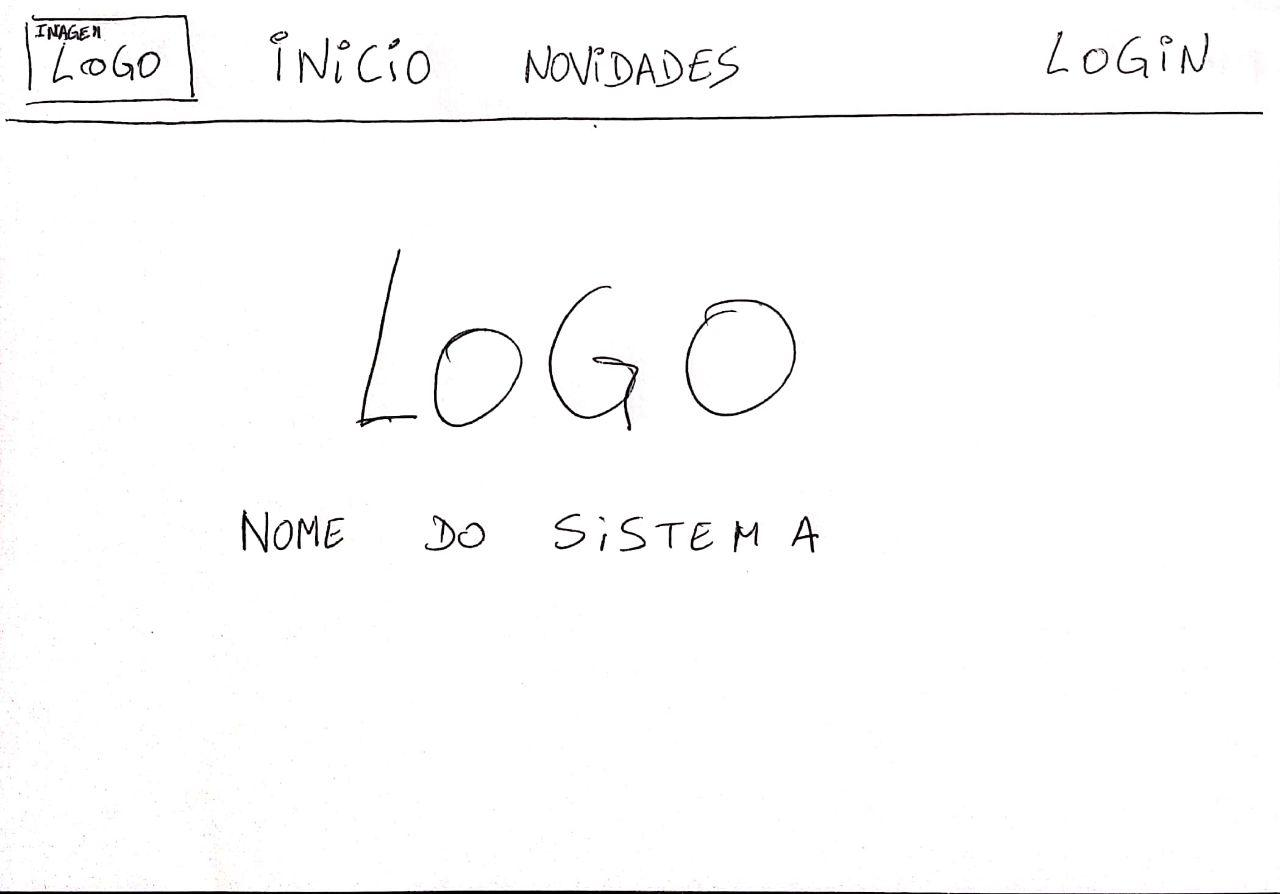
\includegraphics[width=0.5\textwidth, frame]{figuras/storyboard/frame_0.jpg}
	\caption{Desenho de baixa fidelidade da página inicial do portal}
	\label{fig:inicio}
\end{figure}

\FloatBarrier
A figura \ref{fig:login} representa a página de login, onde apenas existem campos de texto para inserir as credenciais de autenticação e o o botão de submissão. Mais uma vez a barra de navegação encontra-se no topo do ecrã.
\begin{figure}[!htb]
	\centering
	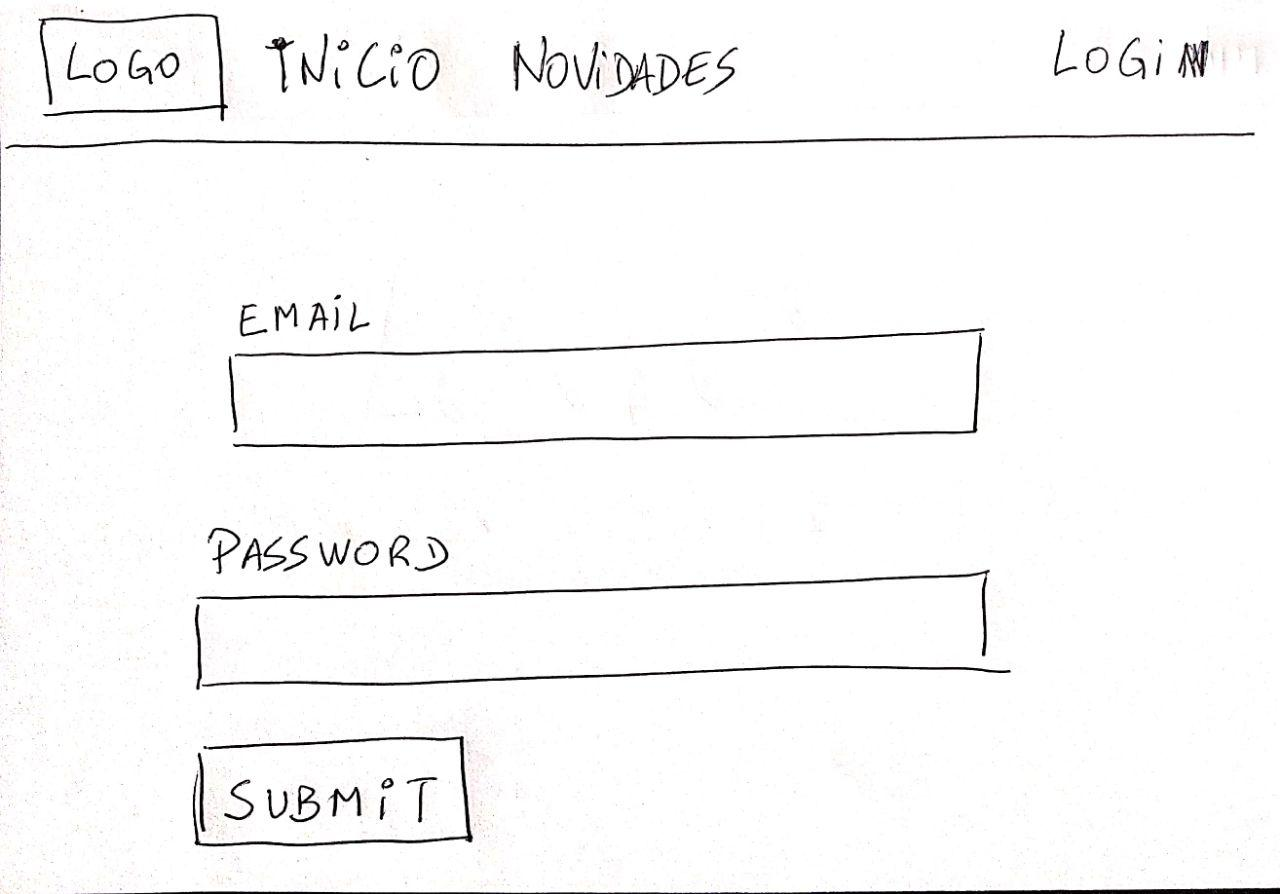
\includegraphics[width=0.5\textwidth, frame]{figuras/storyboard/frame_1.jpg}
	\caption{Desenho de baixa fidelidade da página de login}
	\label{fig:login}
\end{figure}

\FloatBarrier
A figura \ref{fig:novidades} representa a página para a qual um utilizador é levado após o login. Esta página é também acessível a utilizadores não registados. Aqui são apresentadas pequenas noticias ou informações importante relacionadas com o sistemas. Todas estas informações são da responsabilidade do gestor do sistema.
\begin{figure}[!htb]
	\centering
	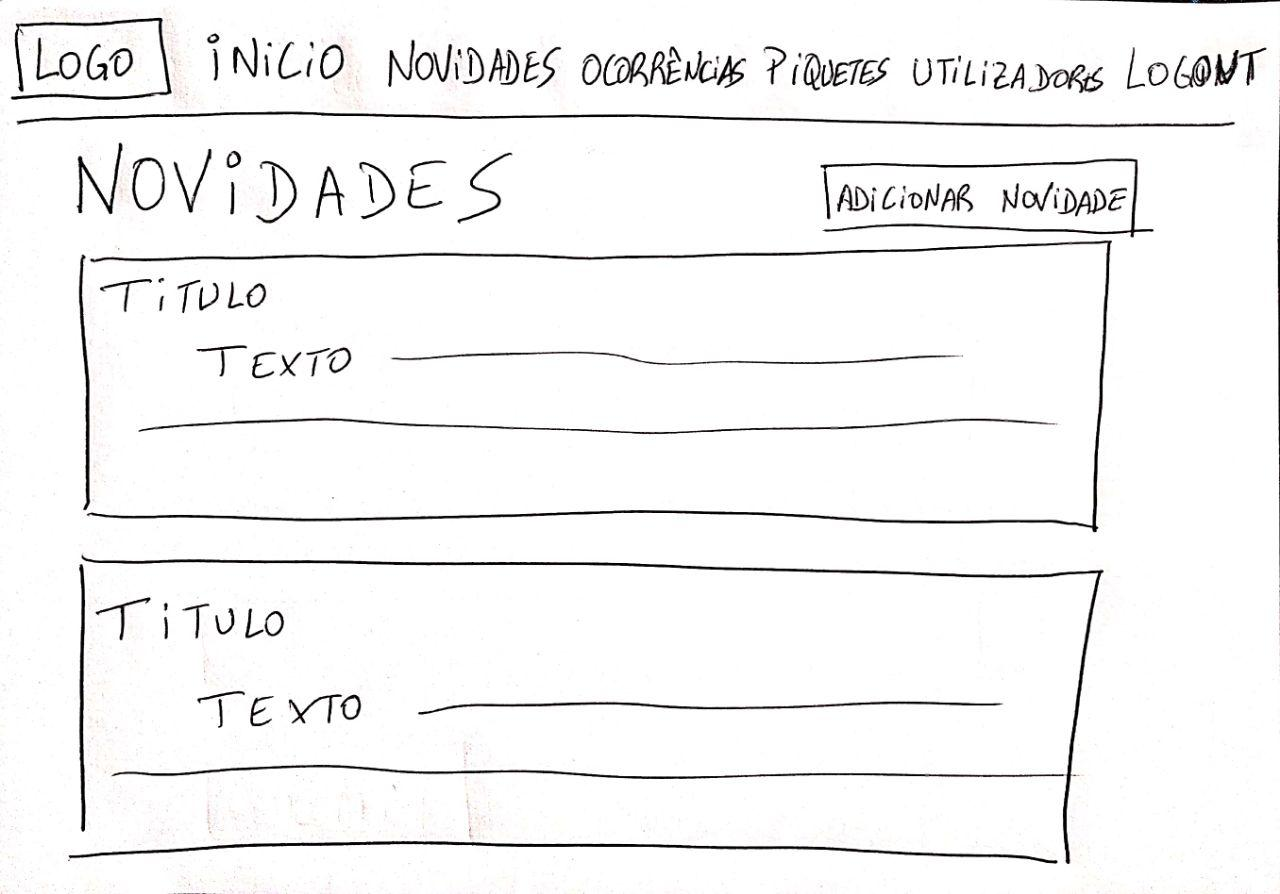
\includegraphics[width=0.5\textwidth, frame]{figuras/storyboard/frame_2.jpg}
	\caption{Desenho de baixa fidelidade da página novidades}
	\label{fig:novidades}
\end{figure}

\FloatBarrier
A figura \ref{fig:adicionar_novidades} representa a página na qual é possível adicionar uma novidade. A novidade é uma mensagem com informação importante para os utilizadores do sistema. Será sempre constituída por um título e mensagem, tendo ainda possibilidade de inserir um link externo.  
\begin{figure}[!htb]
	\centering
	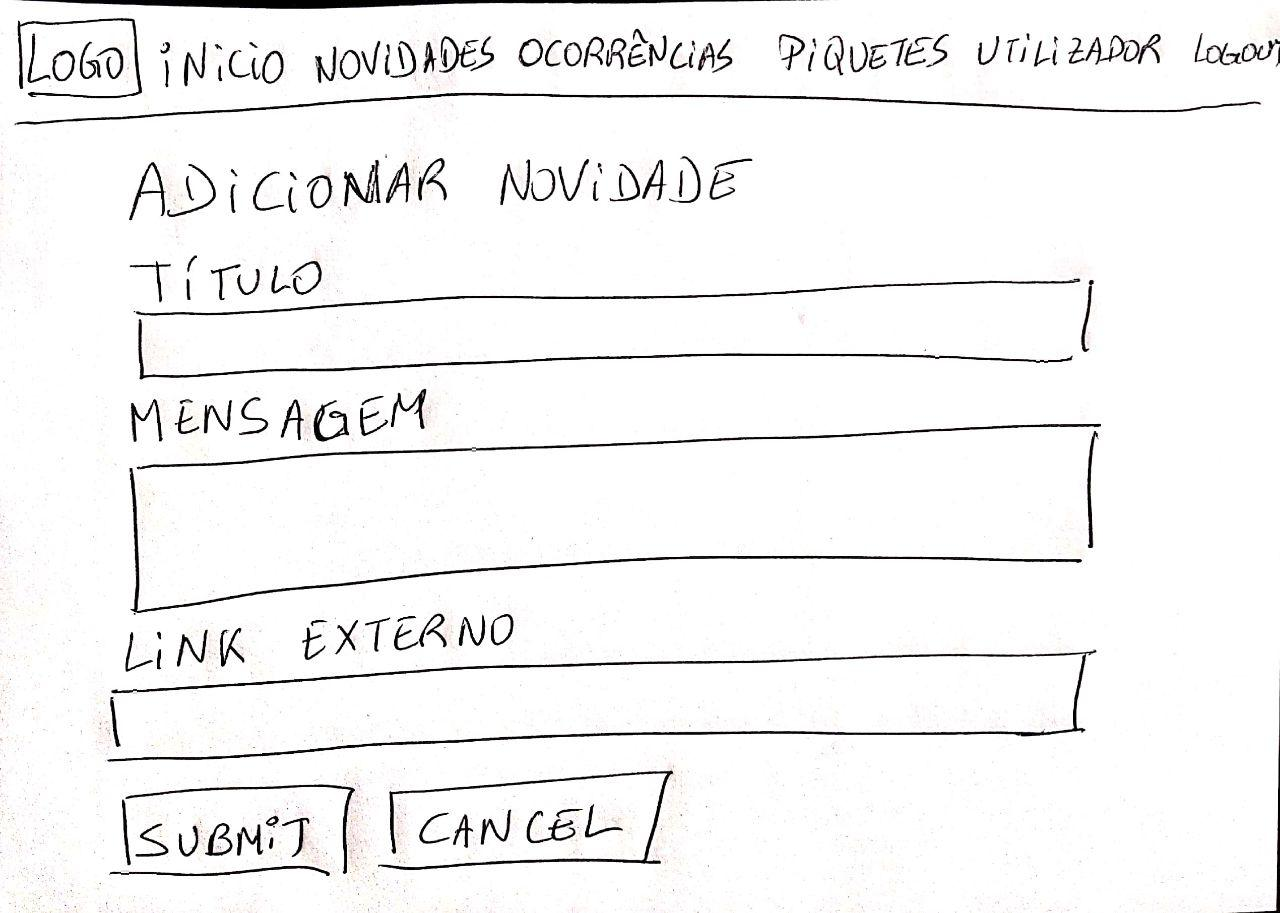
\includegraphics[width=0.5\textwidth, frame]{figuras/storyboard/frame_3.jpg}
	\caption{Desenho de baixa fidelidade da página adicionar novidades}
	\label{fig:adicionar_novidades}
\end{figure}

\FloatBarrier
A figura \ref{fig:ocorrencias} representa a página de ocorrências, onde estão listadas as ocorrências enviadas pelos dispositivos móveis que estão ligado ao portal. A lista é apresentada sob a forma de feed, onde é possível alterar o estado da ocorrência, de modo a assinalar a mesma como resolvida ou não resolvida, ver os detalhes da ocorrência e apagá-la. esta ultima opção poderá estar apenas presente nas versões de teste, pois é útil nesta fase.
\begin{figure}[!htb]
\centering
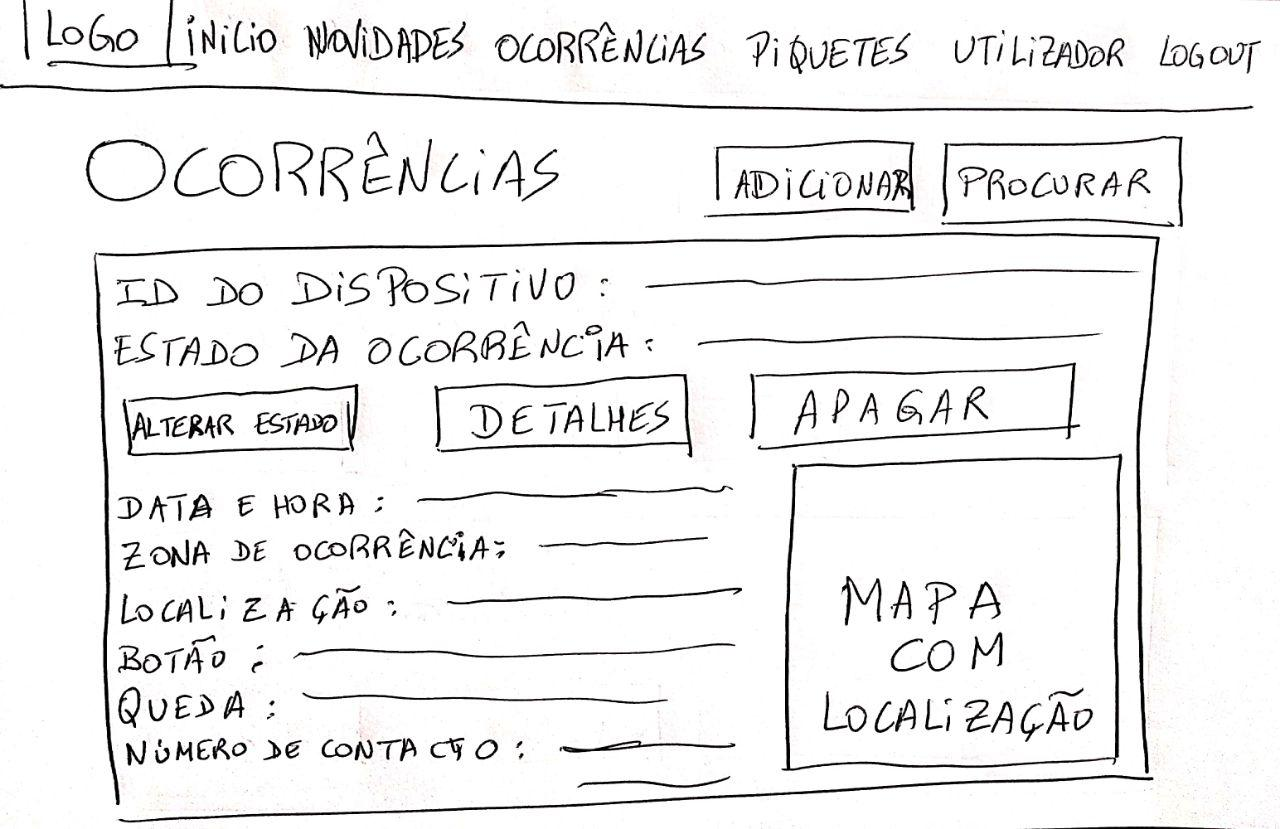
\includegraphics[width=0.5\textwidth, frame]{figuras/storyboard/frame_4.jpg}
\caption{Desenho de baixa fidelidade da página ocorrências}
\label{fig:ocorrencias}
\end{figure}

\FloatBarrier
A figura \ref{fig:ocorrência_detalhes} representa a página de ocorrências com os detalhes de uma ocorrência observáveis. Estas informações são uma mistura de dados enviados pelo dispositivo móvel (data, zona, localização e tipo de sensor activado) e dados já processados pelo portal, uma vez que é este que adiciona o mapa com localização e os números de contacto dos piquetes.
\begin{figure}[!htb]
	\centering
	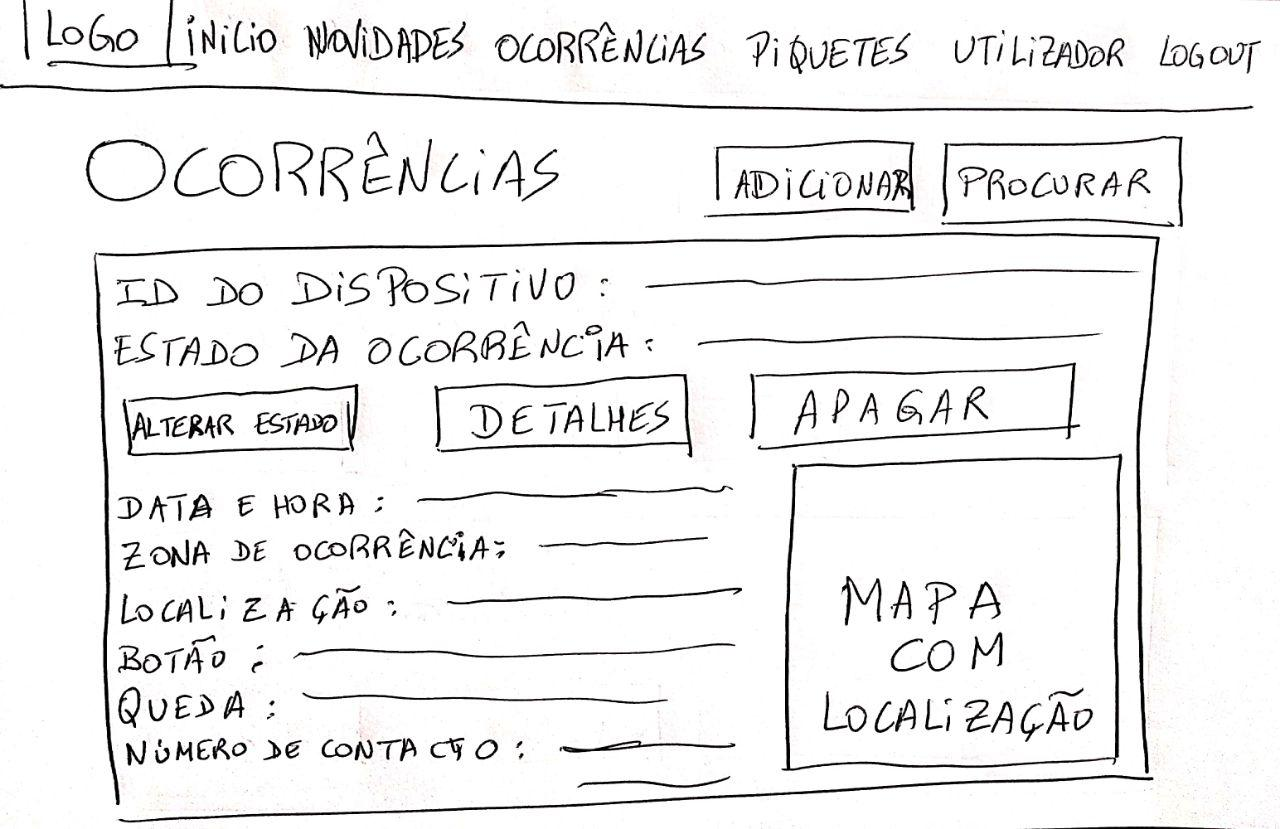
\includegraphics[width=0.5\textwidth, frame]{figuras/storyboard/frame_5.jpg}
	\caption{Desenho de baixa fidelidade da página de detalhes de ocorrência}
	\label{fig:ocorrência_detalhes}
\end{figure}

\FloatBarrier
A figura \ref{fig:piquetes} representa a página de piquetes onde é possível gerir os piquetes já criados, bem como adicionar novos.
\begin{figure}[!htb]
	\centering
	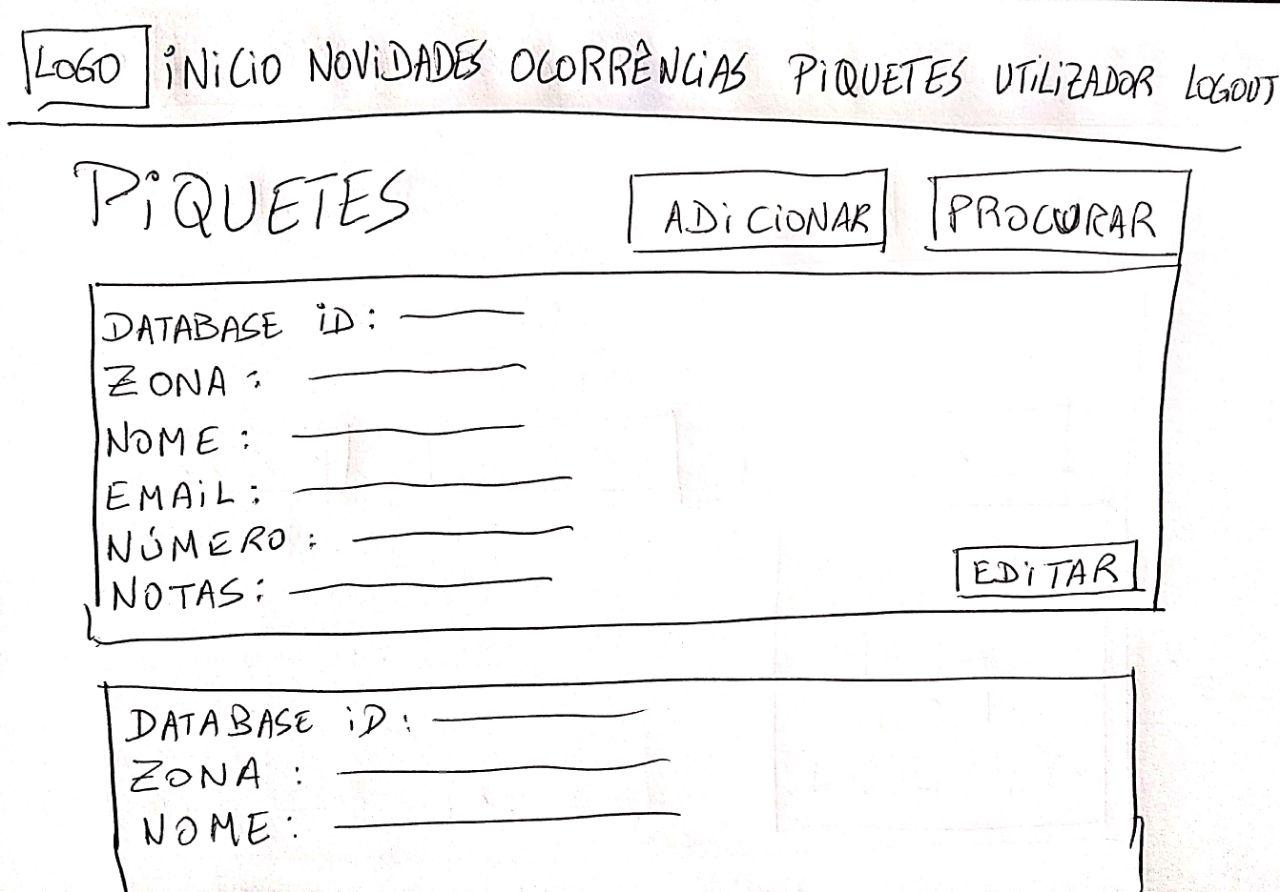
\includegraphics[width=0.5\textwidth, frame]{figuras/storyboard/frame_6.jpg}
	\caption{Desenho de baixa fidelidade da página piquetes}
	\label{fig:piquetes}
\end{figure}

\FloatBarrier
A figura \ref{fig:adicionar_piquetes} representa a página na qual é possível adicionar um piquete. Para tal é necessário preencher os campos de texto com a zona de acção do piquete, nome, email e números de contacto. Será ainda possível adicionar notas sobre o piquete que vamos criar.
\begin{figure}[!htb]
	\centering
	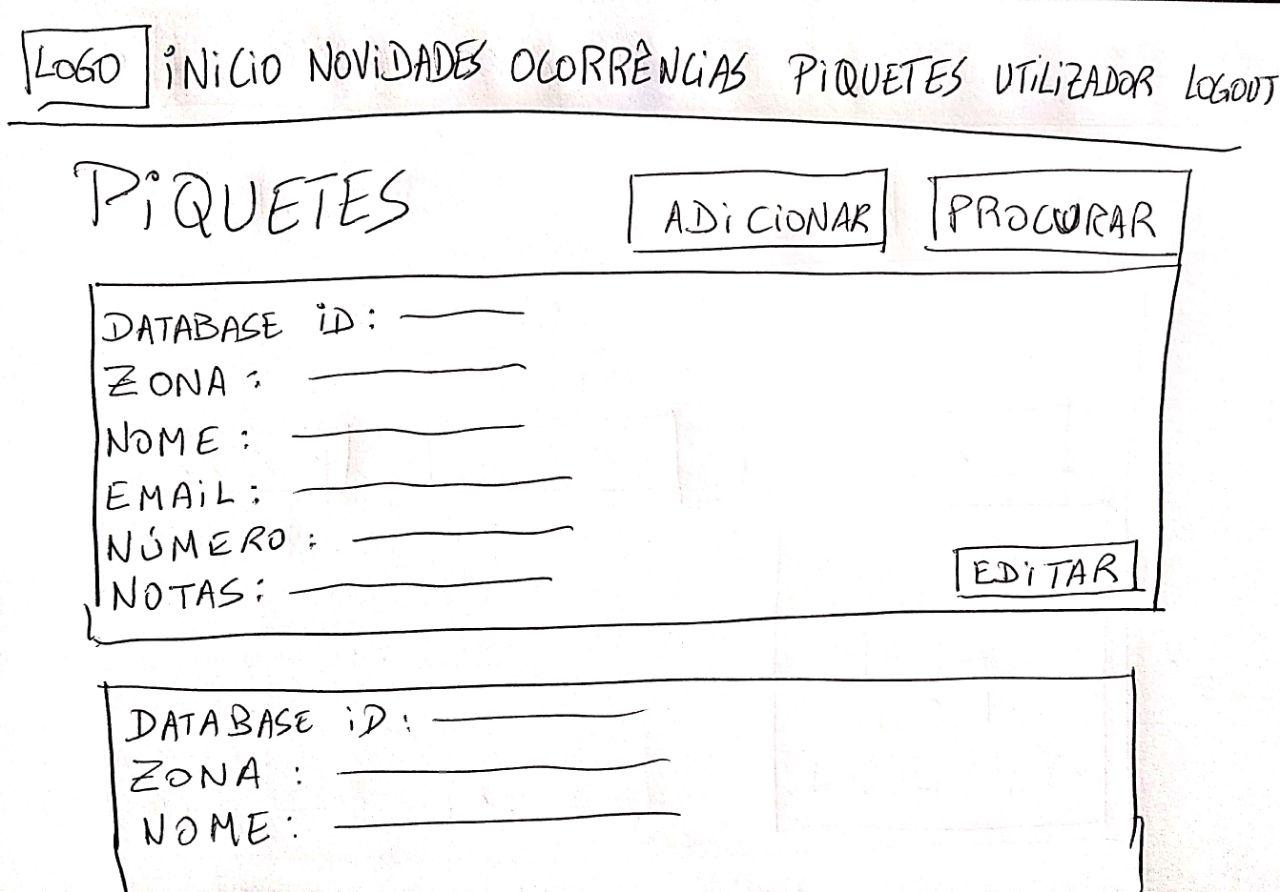
\includegraphics[width=0.5\textwidth, frame]{figuras/storyboard/frame_7.jpg}
	\caption{Desenho de baixa fidelidade da página adicionar piquetes}
	\label{fig:adicionar_piquetes}
\end{figure}

\FloatBarrier
A figura \ref{fig:utilizadores} representa a página de utilizadores
\begin{figure}[!htb]
	\centering
	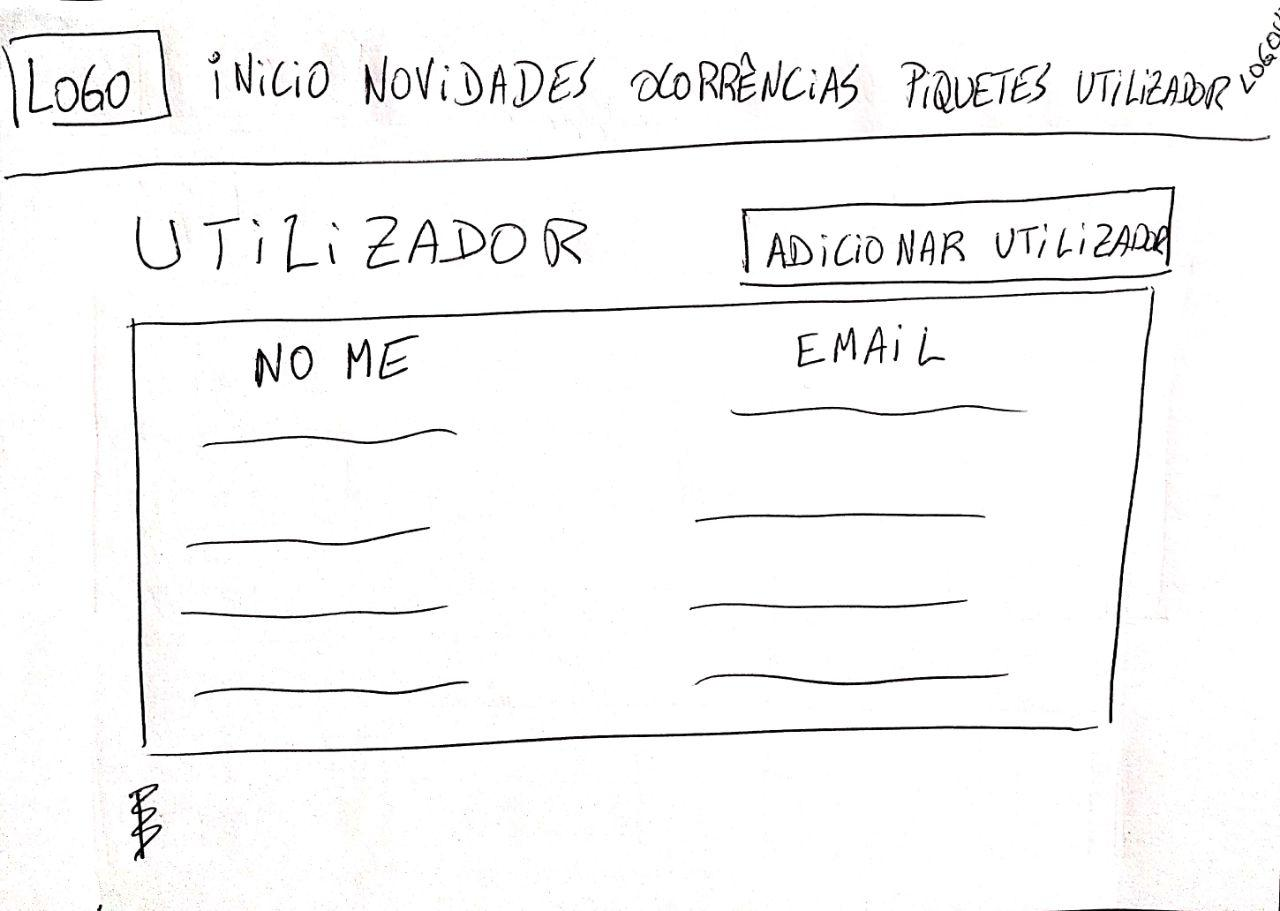
\includegraphics[width=0.5\textwidth, frame]{figuras/storyboard/frame_8.jpg}
	\caption{Desenho de baixa fidelidade da página utilizadores}
	\label{fig:utilizadores}
\end{figure}

%\FloatBarrier\subsection{Interface do caso de uso 1}
%
%%desenhos que descrevem a sequencia do casos de uso 1

\FloatBarrier\section{Modelação da base de dados}

A modelação da base de dados é fundamental para a implementação do sistema de forma correcta, o seu estudo e desenvolvimento são apresentados nos pontos seguintes e a forma como as entidades e classes estão relacionadas permite uma analise da complexidade do sistema, assim sendo, foi possível gerir a complexidade do modelo da base de dados de forma rigorosa. Em seguida são descritos os modelos E/R e físico da base de dados.

\FloatBarrier\subsection{Modelo Entidade-Relação}

A figura \ref{fig:Modelo_E/R} permite observar as relações entre as diversas entidades da base de dados. Através deste diagrama simplificado podemos visualizar as diversas acções que podem ser realizadas sobre o sistema.
O dispositivo, vai actuar como elemento central, uma vez que terá a capacidade de criar a ocorrência, que por sua vez será enviada ao piquete através do portal. Desta forma achamos que podemos garantir um funcionamento rápido e fiável do sistema. O portal, terá como função apresentar as informações ao utilizadores, tendo o gestor a capacidade de criar utilizadores, enquanto que este limitam-se à criação de novidades (pequenos elementos de texto que são apresentados na página inicial). O gestor poderá ainda gerir as listas de ocorrências e piquetes.

\begin{figure}[!htb]
	\centering
	\includegraphics[width=\textwidth]{figuras/diagrama_e-r.png}
	\caption{Modelo entidade-relação}
	\label{fig:Modelo_E/R}
\end{figure}

\FloatBarrier\subsection{Modelo Físico}

O modelo físico, apresentado na figura \ref{fig:Modelo_fisico} complementa o modelo entidade-relação, especificando também os atributos de cada uma das tabelas.

\begin{figure}[!htb]
	\centering
	\includegraphics[width=\textwidth]{figuras/modelo_físico.png}
	\caption{Modelo físico}
	\label{fig:Modelo_fisico}
\end{figure}

\FloatBarrier\section{Modelação UML}

Através da linguagem de modelação unificada (UML) conseguimos representar de uma forma mais padronizada o nosso sistema. Esta linguagem é essencial pois permitiu compreender mais facilmente os passos necessários para a implementação do desenho.

\FloatBarrier\subsection{Diagrama de classes}

A figura \ref{fig:diagrama_classes} representa o diagrama de classes desenvolvido através da fase de desenho. é ainda de salientar que devido à natureza do nosso projecto existem dois elementos diferentes, o dispositivo móvel e o portal. Ambos foram desenhados como se fossem sistemas separados pois possuem as suas classes devidamente independentes.


\begin{figure}[!htb]
	\centering
	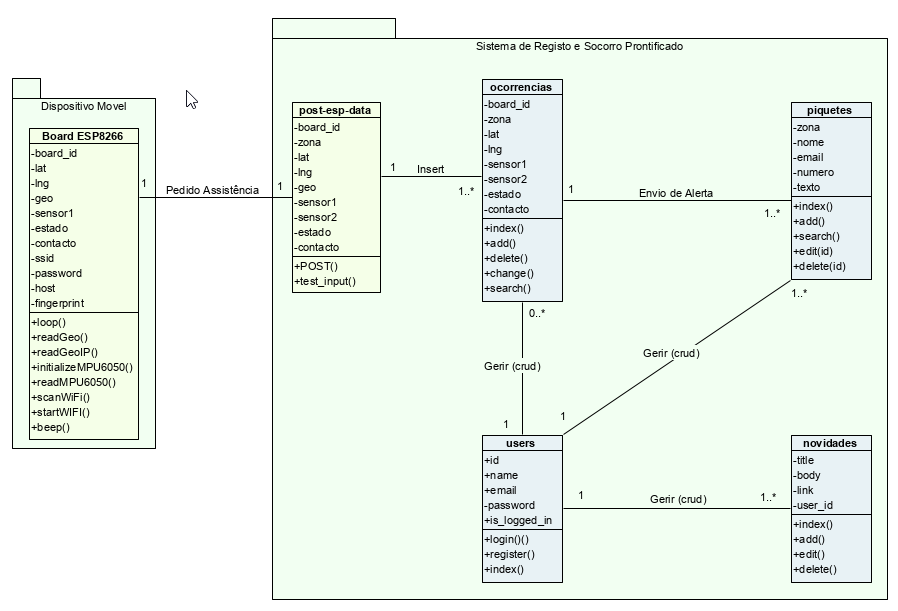
\includegraphics[width=\textwidth]{figuras/diagrama_classes.png}
	\caption{Diagrama de classes}
	\label{fig:diagrama_classes}
\end{figure}

O dispositivo móvel possui apenas uma classe que lhe permite criar uma ligação Wifi, obter a geolocalização ()quer por coordenadas quer através do IP da ligação), inicializar os sensores e ler os valores obtidos pelos sensores. 
existe ainda dentro da classe o método loop, que permite o funcionamento do dispositivo. É neste método que é criada uma string que é enviada ao portal para processamento. Este envio da string é o que nos descrevemos na figura como pedido de assistência.
O portal cinco classes, das quais as classes ocorrências, piquetes, users e novidades são utilizadas para a gestão destas entidades. A classe post-esp-data trata da comunicação da ocorrência ao piquete.

Devido à simplicidade do método que optamos por criar o diagrama de classes não faz um verdadeiro jus à complexidade  da operação do pedido de assistência, pelo que optamos por apresentar também fluxogramas que descrevem o as operações quer do dispositivo móvel, quer do portal.

Assim a figura \ref{fig:fluxograma_ESP} descreve as operações do dispositivo móvel. Existe assim um loop a correr continuamente que verifica em primeiro lufar a ligação à rede wifi, de seguida lê os sensores. Caso haja uma detecção por parte dos sensores é criada uma flag, é obtida a localização (coordenadas ou IP) e é criado um string de post que é enviada ao portal. A flag é então limpa e o loop recomeça.

\begin{figure}[!htb]
	\centering
	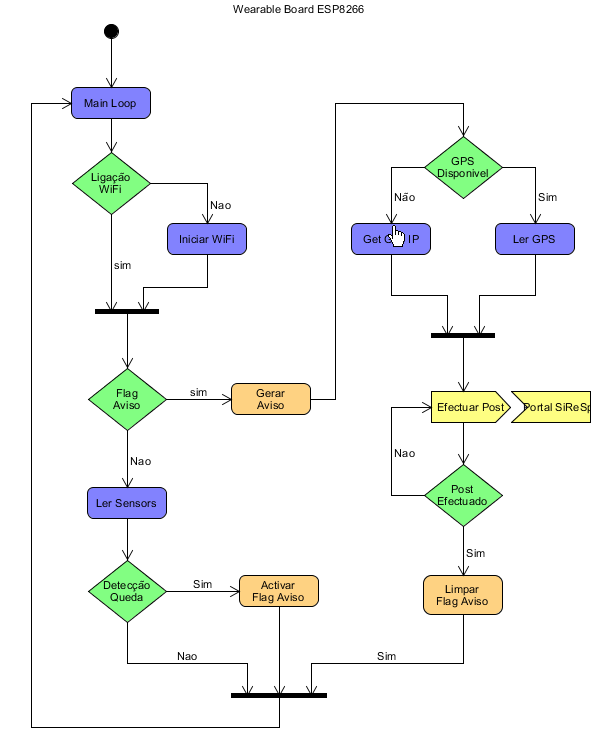
\includegraphics[width=\textwidth]{figuras/fluxograma_ESP.png}
	\caption{Fluxograma do funcionamento do ESP}
	\label{fig:fluxograma_ESP}
\end{figure}

A figura \ref{fig:fluxograma_portal} descreve as operações do portal. Este ao receber a string de post, analisa-a e separa os diferentes campos. Com esta informação cria uma ocorrência na base de dados, consulta a tabela piquetes de modo a seleccionar qual o piquete associado à área geográfica e por fim cria e envia o e-mail ao piquete seleccionado. 

\begin{figure}[!htb]
	\centering
	\includegraphics[width=\textwidth]{figuras/fluxograma_portal.png}
	\caption{Fluxograma do funcionamento do portal}
	\label{fig:fluxograma_portal}
\end{figure}

\FloatBarrier\subsection{Diagrama de sequência}

Os diagramas de sequência servem para demonstrar o funcionamento e interacção entre as classes e os actores. Estes diagrama ajudam-nos a visualizar e validar cenários de utilização, podendo assim ter uma melhor visão do modelo que estamos a criar e ter a possibilidade de prever falhas e comportamentos anómalos.

\FloatBarrier\subsection{Cenário 'adicionar piquete'}

\begin{figure}[!htb]
	\centering
	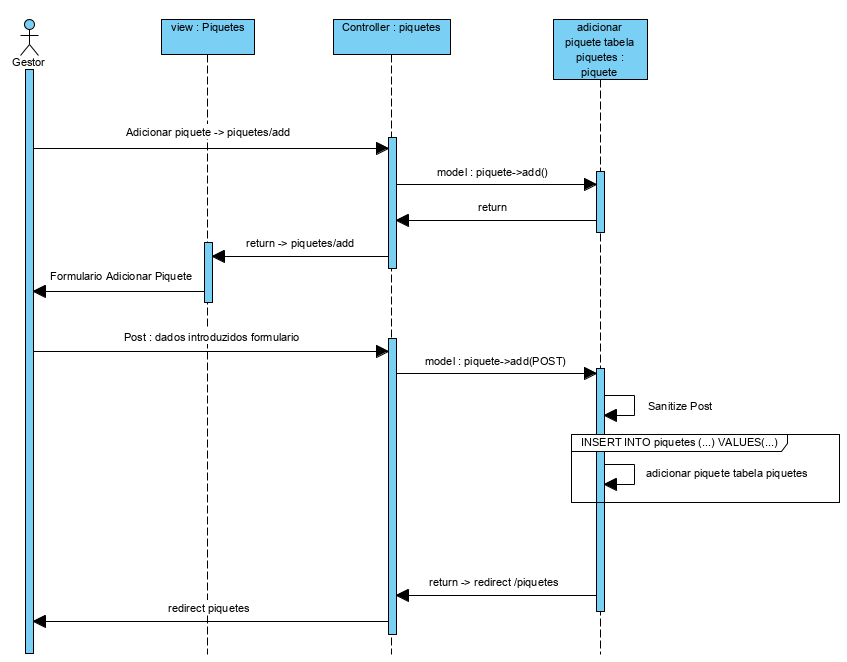
\includegraphics[width=\textwidth]{figuras/sequence_diagram_gestor.png}
	\caption{Diagrama de sequência para o cenário adicionar piquete}
	\label{fig:sequência_gestor}
\end{figure}

\FloatBarrier\subsection{Cenário 'detecção de queda'}

\begin{figure}[!htb]
	\centering
	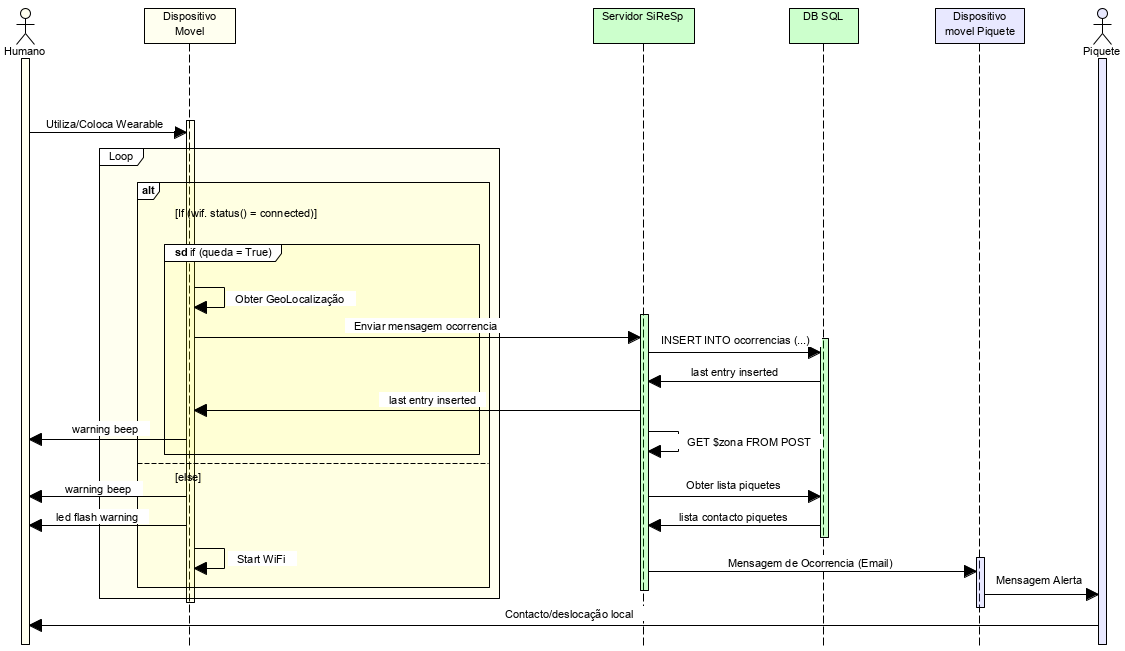
\includegraphics[width=\textwidth]{figuras/sequence_diagram_system_2.png}
	\caption{Diagrama de sequência para o cenário detecção de queda}
	\label{fig:sequência_sistema}
\end{figure}

\FloatBarrier\subsection{Cenário 'VISITANTE'}

\begin{figure}[!htb]
	\centering
	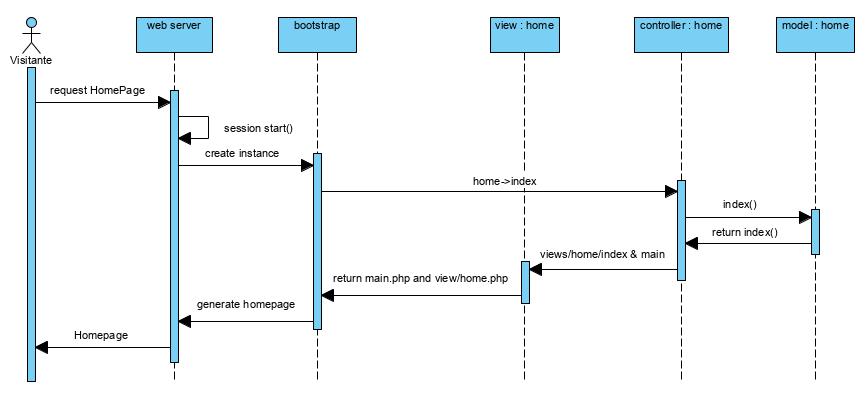
\includegraphics[width=\textwidth]{figuras/sequence_diagram_visitante.png}
	\caption{Diagrama de sequência para ...}
	\label{fig:sequência_visitante}
\end{figure}